% Options for packages loaded elsewhere
\PassOptionsToPackage{unicode}{hyperref}
\PassOptionsToPackage{hyphens}{url}
%
\documentclass[
  ,jou,floatsintext]{apa6}
\usepackage{amsmath,amssymb}
\usepackage{lmodern}
\usepackage{iftex}
\ifPDFTeX
  \usepackage[T1]{fontenc}
  \usepackage[utf8]{inputenc}
  \usepackage{textcomp} % provide euro and other symbols
\else % if luatex or xetex
  \usepackage{unicode-math}
  \defaultfontfeatures{Scale=MatchLowercase}
  \defaultfontfeatures[\rmfamily]{Ligatures=TeX,Scale=1}
\fi
% Use upquote if available, for straight quotes in verbatim environments
\IfFileExists{upquote.sty}{\usepackage{upquote}}{}
\IfFileExists{microtype.sty}{% use microtype if available
  \usepackage[]{microtype}
  \UseMicrotypeSet[protrusion]{basicmath} % disable protrusion for tt fonts
}{}
\makeatletter
\@ifundefined{KOMAClassName}{% if non-KOMA class
  \IfFileExists{parskip.sty}{%
    \usepackage{parskip}
  }{% else
    \setlength{\parindent}{0pt}
    \setlength{\parskip}{6pt plus 2pt minus 1pt}}
}{% if KOMA class
  \KOMAoptions{parskip=half}}
\makeatother
\usepackage{xcolor}
\usepackage{graphicx}
\makeatletter
\def\maxwidth{\ifdim\Gin@nat@width>\linewidth\linewidth\else\Gin@nat@width\fi}
\def\maxheight{\ifdim\Gin@nat@height>\textheight\textheight\else\Gin@nat@height\fi}
\makeatother
% Scale images if necessary, so that they will not overflow the page
% margins by default, and it is still possible to overwrite the defaults
% using explicit options in \includegraphics[width, height, ...]{}
\setkeys{Gin}{width=\maxwidth,height=\maxheight,keepaspectratio}
% Set default figure placement to htbp
\makeatletter
\def\fps@figure{htbp}
\makeatother
\setlength{\emergencystretch}{3em} % prevent overfull lines
\providecommand{\tightlist}{%
  \setlength{\itemsep}{0pt}\setlength{\parskip}{0pt}}
\setcounter{secnumdepth}{-\maxdimen} % remove section numbering
% Make \paragraph and \subparagraph free-standing
\ifx\paragraph\undefined\else
  \let\oldparagraph\paragraph
  \renewcommand{\paragraph}[1]{\oldparagraph{#1}\mbox{}}
\fi
\ifx\subparagraph\undefined\else
  \let\oldsubparagraph\subparagraph
  \renewcommand{\subparagraph}[1]{\oldsubparagraph{#1}\mbox{}}
\fi
\newlength{\cslhangindent}
\setlength{\cslhangindent}{1.5em}
\newlength{\csllabelwidth}
\setlength{\csllabelwidth}{3em}
\newlength{\cslentryspacingunit} % times entry-spacing
\setlength{\cslentryspacingunit}{\parskip}
\newenvironment{CSLReferences}[2] % #1 hanging-ident, #2 entry spacing
 {% don't indent paragraphs
  \setlength{\parindent}{0pt}
  % turn on hanging indent if param 1 is 1
  \ifodd #1
  \let\oldpar\par
  \def\par{\hangindent=\cslhangindent\oldpar}
  \fi
  % set entry spacing
  \setlength{\parskip}{#2\cslentryspacingunit}
 }%
 {}
\usepackage{calc}
\newcommand{\CSLBlock}[1]{#1\hfill\break}
\newcommand{\CSLLeftMargin}[1]{\parbox[t]{\csllabelwidth}{#1}}
\newcommand{\CSLRightInline}[1]{\parbox[t]{\linewidth - \csllabelwidth}{#1}\break}
\newcommand{\CSLIndent}[1]{\hspace{\cslhangindent}#1}
\ifLuaTeX
\usepackage[bidi=basic]{babel}
\else
\usepackage[bidi=default]{babel}
\fi
\babelprovide[main,import]{english}
% get rid of language-specific shorthands (see #6817):
\let\LanguageShortHands\languageshorthands
\def\languageshorthands#1{}
% Manuscript styling
\usepackage{upgreek}
\captionsetup{font=singlespacing,justification=justified}

% Table formatting
\usepackage{longtable}
\usepackage{lscape}
% \usepackage[counterclockwise]{rotating}   % Landscape page setup for large tables
\usepackage{multirow}		% Table styling
\usepackage{tabularx}		% Control Column width
\usepackage[flushleft]{threeparttable}	% Allows for three part tables with a specified notes section
\usepackage{threeparttablex}            % Lets threeparttable work with longtable

% Create new environments so endfloat can handle them
% \newenvironment{ltable}
%   {\begin{landscape}\centering\begin{threeparttable}}
%   {\end{threeparttable}\end{landscape}}
\newenvironment{lltable}{\begin{landscape}\centering\begin{ThreePartTable}}{\end{ThreePartTable}\end{landscape}}

% Enables adjusting longtable caption width to table width
% Solution found at http://golatex.de/longtable-mit-caption-so-breit-wie-die-tabelle-t15767.html
\makeatletter
\newcommand\LastLTentrywidth{1em}
\newlength\longtablewidth
\setlength{\longtablewidth}{1in}
\newcommand{\getlongtablewidth}{\begingroup \ifcsname LT@\roman{LT@tables}\endcsname \global\longtablewidth=0pt \renewcommand{\LT@entry}[2]{\global\advance\longtablewidth by ##2\relax\gdef\LastLTentrywidth{##2}}\@nameuse{LT@\roman{LT@tables}} \fi \endgroup}

% \setlength{\parindent}{0.5in}
% \setlength{\parskip}{0pt plus 0pt minus 0pt}

% Overwrite redefinition of paragraph and subparagraph by the default LaTeX template
% See https://github.com/crsh/papaja/issues/292
\makeatletter
\renewcommand{\paragraph}{\@startsection{paragraph}{4}{\parindent}%
  {0\baselineskip \@plus 0.2ex \@minus 0.2ex}%
  {-1em}%
  {\normalfont\normalsize\bfseries\itshape\typesectitle}}

\renewcommand{\subparagraph}[1]{\@startsection{subparagraph}{5}{1em}%
  {0\baselineskip \@plus 0.2ex \@minus 0.2ex}%
  {-\z@\relax}%
  {\normalfont\normalsize\itshape\hspace{\parindent}{#1}\textit{\addperi}}{\relax}}
\makeatother

% \usepackage{etoolbox}
\makeatletter
\patchcmd{\HyOrg@maketitle}
  {\section{\normalfont\normalsize\abstractname}}
  {\section*{\normalfont\normalsize\abstractname}}
  {}{\typeout{Failed to patch abstract.}}
\patchcmd{\HyOrg@maketitle}
  {\section{\protect\normalfont{\@title}}}
  {\section*{\protect\normalfont{\@title}}}
  {}{\typeout{Failed to patch title.}}
\makeatother

\usepackage{xpatch}
\makeatletter
\xapptocmd\appendix
  {\xapptocmd\section
    {\addcontentsline{toc}{section}{\appendixname\ifoneappendix\else~\theappendix\fi\\: #1}}
    {}{\InnerPatchFailed}%
  }
{}{\PatchFailed}
\usepackage{dblfloatfix}


\usepackage{csquotes}
\ifLuaTeX
  \usepackage{selnolig}  % disable illegal ligatures
\fi
\IfFileExists{bookmark.sty}{\usepackage{bookmark}}{\usepackage{hyperref}}
\IfFileExists{xurl.sty}{\usepackage{xurl}}{} % add URL line breaks if available
\urlstyle{same} % disable monospaced font for URLs
\hypersetup{
  pdftitle={Faith in Reason: developing a survey measure of belief in the rationality of others},
  pdfauthor={Tom Stafford1, Junyan Zhu2, \& Katharine Dommett2},
  pdflang={en-EN},
  hidelinks,
  pdfcreator={LaTeX via pandoc}}

\title{Faith in Reason: developing a survey measure of belief in the rationality of others}
\author{Tom Stafford\textsuperscript{1}, Junyan Zhu\textsuperscript{2}, \& Katharine Dommett\textsuperscript{2}}
\date{}


\shorttitle{Faith in Reason}

\authornote{

For the purpose of open access, the author has applied a Creative Commons Attribution (CC BY) licence to any Author Accepted Manuscript version arising.

Document prepared with RMarkdown (Allaire et al., 2020) and papaja (Aust \& Barth, 2020). CRediT (Contributor Roles Taxonomy) autogenerated using Tenzing (Holcombe, Kovacs, Aust, \& Aczel, 2020). Template is available here \href{https://github.com/tomstafford/rmarkdown_apa}{github.com/tomstafford/rmarkdown\_apa}

The authors made the following contributions. Tom Stafford: Conceptualization, Data curation, Formal analysis, Funding acquisition, Methodology, Visualization, Writing - original draft, Writing - review \& editing; Junyan Zhu: Conceptualization, Data curation, Formal analysis, Methodology, Visualization, Writing - original draft, Writing - review \& editing; Katharine Dommett: Conceptualization, Funding acquisition, Methodology, Writing - review \& editing.

Correspondence concerning this article should be addressed to Tom Stafford, Department of Psychology, University of Sheffield, Sheffield, UK. E-mail: \href{mailto:t.stafford@sheffield.ac.uk}{\nolinkurl{t.stafford@sheffield.ac.uk}}

}

\affiliation{\vspace{0.5cm}\textsuperscript{1} Department of Psychology, University of Sheffield, UK\\\textsuperscript{2} Department of Politics and International Relations, University of Sheffield, UK}

\note{\textcolor{red}{Preprint 2023-02-20}}

\abstract{%
abstract goes here
}



\begin{document}
\maketitle

\hypertarget{introduction}{%
\section{Introduction}\label{introduction}}

\hypertarget{method}{%
\section{Method}\label{method}}

Rmarkdown also lets us track figure labels, and updates them automatically. Look! Kittens! Illustrated in Figure \ref{fig:examplefigurename}. And if I add other figures it will sort out the numbering and references automatically

\hypertarget{results}{%
\section{Results}\label{results}}

Now let's integrate some R code to generate/import some data, run and analyse and integrate it into the document:

You can't see it in the PDF, but in between this paragraph and the last we asked R to generate some random data and save it to a CSV file. Now we're going to import the data from the CSV file, as if it was independently created data - from an experiment or similar - and plot a graph.

\begin{figure}

{\centering 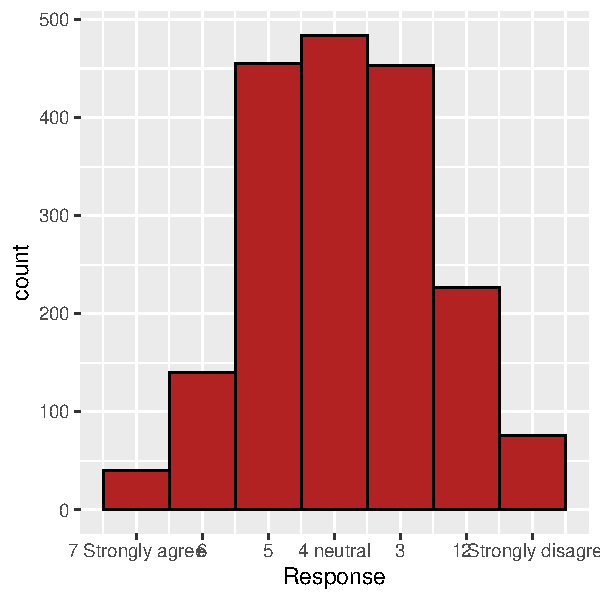
\includegraphics[width=0.75\linewidth]{faithinreason_files/figure-latex/ourhistogram-1} 

}

\caption{Histogram of all data, grouped}\label{fig:ourhistogram}
\end{figure}

See Figure \ref{fig:ourhistogram}. Of course we could draw all sorts of things, but this is a proof-of-concept. Finally, let's run a t-test and integrate the results into the text.

We found there was a statistically significant difference between the two groups (t=-6.00 (588.26), p = 0.00). Note how the exact values in the previous sentence change every time we re-make the document (because the document also re-generates the underlying data).

The above paragraph does the integration of statistics longform, because I didn't know a better way (and because I think it is still useful to show). apa\_print() exists as a helper function: \url{http://frederikaust.com/papaja_man/reporting.html}.

\begin{table}[tbp]

\begin{center}
\begin{threeparttable}

\caption{\label{tab:asrssub}Item grouping to subscales}

\begin{tabular}{lll}
\toprule
 & \multicolumn{1}{c}{Hyperactivity} & \multicolumn{1}{c}{Inattention}\\
\midrule
ASRS-18 & 5,6,12,13,14 & 1,2,3,4,7,8\\
ASRS-6 & 5,6 & 1,2,3,4\\
\bottomrule
\addlinespace
\end{tabular}

\begin{tablenotes}[para]
\normalsize{\textit{Note.} This table was created with apa\_table().}
\end{tablenotes}

\end{threeparttable}
\end{center}

\end{table}

Also, everyone loves tables. See Table \ref{tab:asrssub}. I feel obliged to mention that the actual items reported in this table \textbf{do not} correctly reflect the actual subscales for the ASRS short and long scales. Note illustration of \textbf{bold} and \emph{italics} formatting in this para.

\hypertarget{discussion}{%
\section{Discussion}\label{discussion}}

\hypertarget{references}{%
\section*{References}\label{references}}
\addcontentsline{toc}{section}{References}

\hypertarget{refs}{}
\begin{CSLReferences}{1}{0}
\leavevmode\vadjust pre{\hypertarget{ref-rmarkdowncite}{}}%
Allaire, J., Xie, Y., McPherson, J., Luraschi, J., Ushey, K., Atkins, A., \ldots{} Iannone, R. (2020). \emph{Rmarkdown: Dynamic documents for r}. Retrieved from \url{https://github.com/rstudio/rmarkdown}

\leavevmode\vadjust pre{\hypertarget{ref-aust2020}{}}%
Aust, F., \& Barth, M. (2020). \emph{{papaja}: {Create} {APA} manuscripts with {R Markdown}}. Retrieved from \url{https://github.com/crsh/papaja}

\leavevmode\vadjust pre{\hypertarget{ref-holcombe2020documenting}{}}%
Holcombe, A. O., Kovacs, M., Aust, F., \& Aczel, B. (2020). Documenting contributions to scholarly articles using CRediT and tenzing. \emph{PLoS One}, \emph{15}(12), e0244611.

\end{CSLReferences}


\end{document}
